\documentclass[10pt,letterpaper,fleqn,titlepage]{article}

% Define packages to use
\usepackage[letterpaper,top=0.85in,bottom=0.75in,left=0.75in,right=0.75in]{geometry}
%\usepackage{natbib}
%\bibliographystyle{plainnat}
\usepackage{graphicx,color}
\usepackage{subcaption}
\usepackage{amsmath,amssymb}
\usepackage{bm}
\usepackage{caption}
\usepackage{xr}
\usepackage{ifthen}
\usepackage[colorlinks,linkcolor=blue,citecolor=blue,urlcolor=blue]{hyperref}
\usepackage{fancybox}
\usepackage{textcomp}
\usepackage{fancyhdr}
\usepackage{alltt}
\usepackage{float}
\usepackage{svn}
\usepackage{longtable}
\usepackage{array}


% Some new columntypes to allow fixed widths but
% with alignment the same as the regular c,l,r
% (requires array package). An example:
%   \begin{tabular}{C{2cm} *{3}{R{1cm}@{.}L{2cm}}}
\newcolumntype{C}[1]{>{\centering\arraybackslash}p{#1}}
\newcolumntype{L}[1]{>{\raggedright\arraybackslash}p{#1}}
\newcolumntype{R}[1]{>{\raggedleft\arraybackslash}p{#1}}

% Redefine default paragraph
\setlength{\parindent}{0pt}
\setlength{\parskip}{1ex plus 0.5ex minus 0.2ex}

% Define caption width and default fonts
\setlength{\captionmargin}{0.5in}
\renewcommand{\captionfont}{\sffamily}
\renewcommand{\captionlabelfont}{\bfseries\sffamily}

% Define commands for super- and subscript in text mode
\newcommand{\superscript}[1]{\ensuremath{^\textrm{#1}}}
\newcommand{\subscript}[1]{\ensuremath{_\textrm{#1}}}

% Derived commands
\newcommand{\invcm}{\textrm{cm\superscript{-1}}}
\newcommand{\micron}{\ensuremath{\mu\textrm{m}}}

\newcommand{\df}{\ensuremath{\delta f}}
\newcommand{\Df}{\ensuremath{\Delta f}}
\newcommand{\dx}{\ensuremath{\delta x}}
\newcommand{\Dx}{\ensuremath{X_{max}}}
\newcommand{\Xeff}{\ensuremath{X_{eff}}}

\newcommand{\water}{\textrm{H\subscript{2}O}}
\newcommand{\carbondioxide}{\textrm{CO\subscript{2}}}
\newcommand{\ozone}{\textrm{O\subscript{3}}}

\newcommand{\taup}[1]{\ensuremath{\tau_{#1}}}
\newcommand{\efftaup}[1]{\ensuremath{\tau_{#1}^{*}}}

\newcommand{\textbfm}[1]{\boldmath\ensuremath{#1}\unboldmath}

\newcommand{\rb}[1]{\raisebox{1.5ex}[0pt]{#1}}

\newcommand{\f}[1]{\texttt{#1}}

\newcommand{\ud}{\,\mathrm{d}}  % differential in integral is conventionally set in upright.

% Define how equations are numbered
\numberwithin{equation}{section}
\numberwithin{figure}{section}
\numberwithin{table}{section}

% Define a command for title page author email footnote
\newcommand{\email}[1]
{%
  \renewcommand{\thefootnote}{\alph{footnote}}%
  \footnote{#1}
  \renewcommand{\thefootnote}{\arabic{footnote}}
}

% Define a command to print the Office Note subheading
\newcommand{\notesubheading}[1]
{%
  \ifthenelse{\equal{#1}{}}{}
  { 
    {\scriptsize \sc This is an unreviewed manuscript}\\ 
  }
}

% Redefine the maketitle macro
\makeatletter
\def\docseries#1{\def\@docseries{#1}}
\def\docnumber#1{\def\@docnumber{#1}}
\renewcommand{\maketitle}
{%
  \thispagestyle{empty}
  \vspace*{1in}
  \begin{center}%
     \sffamily
     {\huge\bfseries Joint Center for Satellite Data Assimilation\par}%
     \notesubheading{CRTM-\@docnumber}
  \end{center}
  \begin{flushleft}%
     \sffamily
     \vspace*{0.5in}
     {\Large\bfseries\ifthenelse{\equal{\@docseries}{}}{}{\@docseries: }\@title\par}%
     \medskip
     {\large\@author\par}%
     \medskip
     {\large\@date\par}%
     \bigskip\hrule\vspace*{2pc}%
  \end{flushleft}%
  \newpage
  \setcounter{footnote}{0}
}
\makeatother
\docseries{}
\docnumber{}


% Define command for watermarking, with a DRAFT specific one
% \usepackage{eso-pic}
% \newcommand{\watermark}[1]
% {
%   \AddToShipoutPicture{%
%     \definecolor{lightgray}{gray}{.85}
%     \setlength{\unitlength}{1in}
%     \put(2.5,3.5){%
%       \rotatebox{45}{%
%         \resizebox{4in}{1in}{%
%           \textsf{\textcolor{lightgray}{#1}}
%         }
%       }
%     }
%   }
% }
% \newcommand{\draftwatermark}{\watermark{DRAFT}}




% Title info
\title{MWI EPS-SG CRTM Coefficients: Boxcar v1}
\author{Dr. Patrick Stegmann\ - \emph{JCSDA},\\ Veljko Petkovic - \emph{University of Maryland}}
\date{\today}
\docnumber{(unassigned)}
\docseries{CRTM}


%-------------------------------------------------------------------------------
%                            Ze document begins...
%-------------------------------------------------------------------------------
\begin{document}

\maketitle

\draftwatermark

\tableofcontents

\newpage

% The front matter
%=================
\thispagestyle{empty}
\vspace*{10cm}
\begin{center}
  {\sffamily\Large\bfseries Change History}
  \begin{table}[htp]
    \centering
    \begin{tabular}{|p{2cm}|p{3cm}|p{8cm}|}
      \hline
      \sffamily\textbf{Date} & \sffamily\textbf{Author} & \sffamily\textbf{Change}\\
      \hline\hline
      2022-01-1 & P. Stegmann& Initial Draft.\\
      \hline
    \end{tabular}
  \end{table}
\end{center}
\clearpage
\pagenumbering{arabic}
\setcounter{page}{1}


% The main matter
%================
%\include{}

\section{Introduction}
The Microwave Imager (MWI) onboard the EUMETSAT Polar System - Second Generation (EPS-SG) is an instrument onboard a polar-orbiting satellite that is designed by EUMETSAT for the timeframe beyond 2022 \cite{mwi}.
The CRTM coefficient implementation of this instrument is a first guess for research applications at the University of Maryland. More refined coefficients will likely be released later on, once additional details about the instrument are known.

\section{Channel Assumptions}
The table below summarizes the assumption about the channel layout taken from Ref. \cite{mwi}. A particularity of the MWI instrument is that the first 8 channels are dual polarization channels, i.e. both horizontal and vertical linear polarization are measured at the same time for these channels. It is currently not possible to simulate this with the CRTM, so the easiest solution is to provide two separate sets of SpcCoeff files, one for each polarization.
The listed bandwidths are the total bandwidths for each channel, viz. a channel is only one bandwidth wide, not twice the bandwidth on either side of the center frequency.
\begin{table}[h!]
\begin{center}
\begin{tabular}{ l | c | c | c }
 Channel & Frequency [GHz] & Bandwidth [MHz] & Polarization\\ 
 \hline \hline
 MWI-1 & 18.7 & 200 & VL + HL \\
 MWI-2 & 23.8 & 400 & VL + HL\\  
 MWI-3 & 31.4 & 200 & VL + HL\\  
 MWI-4 & 50.3 & 400 & VL + HL\\  
 MWI-5 & 52.610 & 400 & VL + HL\\  
 MWI-6 & 53.24 & 400 & VL + HL\\  
 MWI-7 & 53.750 & 400 & VL + HL\\  
 MWI-8 & 89.0 & 4000  & VL + HL\\  
 MWI-9 & 118.7503+/-3.20 & 2 x 500 & VL\\  
 MWI-10 & 118.7503+/-2.10 & 2 x 400 & VL\\  
 MWI-11 & 118.7503+/-1.40 & 2 x 400 & VL\\  
 MWI-12 & 118.7503+/-1.20 & 2 x 400 & VL\\  
 MWI-13 & 165.5+/-0.75 & 2 x 1350 & VL\\  
 MWI-14 & 183.31+/-7.0 & 2 x 2000 & VL\\  
 MWI-15 & 183.31+/-6.1 & 2 x 1500 & VL\\  
 MWI-16 & 183.31+/-4.9 & 2 x 1500 & VL\\  
 MWI-17 & 183.31+/-3.4 & 2 x 1500 & VL\\    
 MWI-18 & 183.31+/-2.0 & 2 x 1500 & VL 
\end{tabular}
 \caption{Channel data for MWI EPS-SG.}
 \label{tab:channels}
\end{center}
\end{table}

\section{Spectral Response Function Assumptions}

Since the instrument is in the planning stage and no precise SRF measurements are yet available, the SRF data for the CRTM instrument coefficients was estimated as a collection of boxcar SRFs based on the channel center frequencies and bandwidths listed in table \ref{tab:channels}. 
The corresponding SRFs can be seen in Figs. \ref{fig:boxcar1} to \ref{fig:boxcar3}.

 \begin{figure}[H]
 \centering
 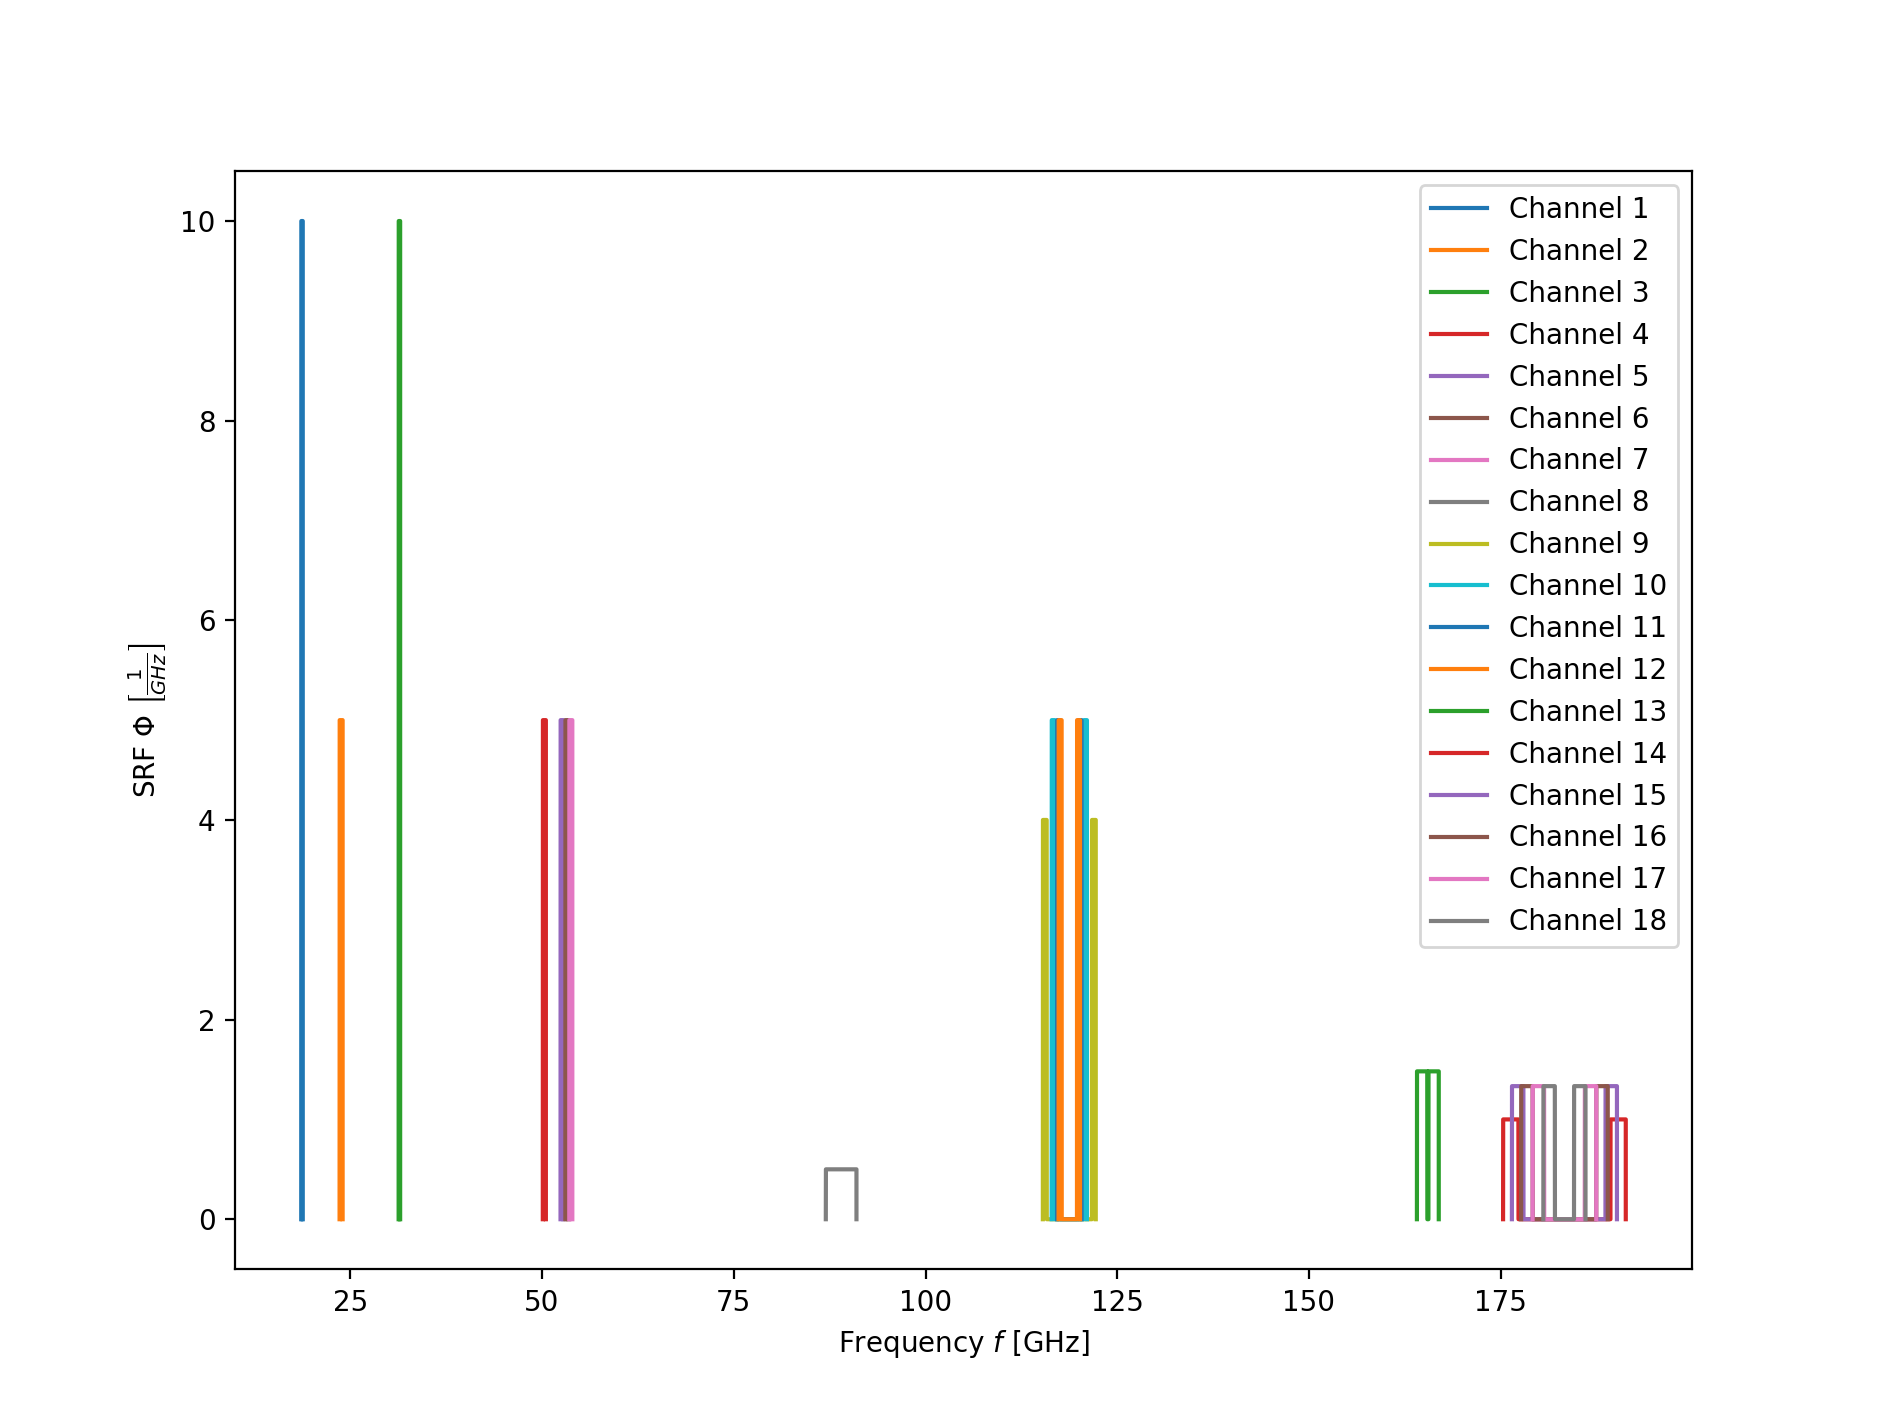
\includegraphics[width=\textwidth]{graphics/mwi-boxcar.png}
 \caption{Boxcar SRFs for all channels of EPS-SG MWI.}
 \label{fig:boxcar1}
 \end{figure}
 
 Fig. \ref{fig:boxcar2} shows a zoom on the SRF of channel 13, which consists of two symmetric bands around the center frequency.
 
  \begin{figure}[H]
 \centering
 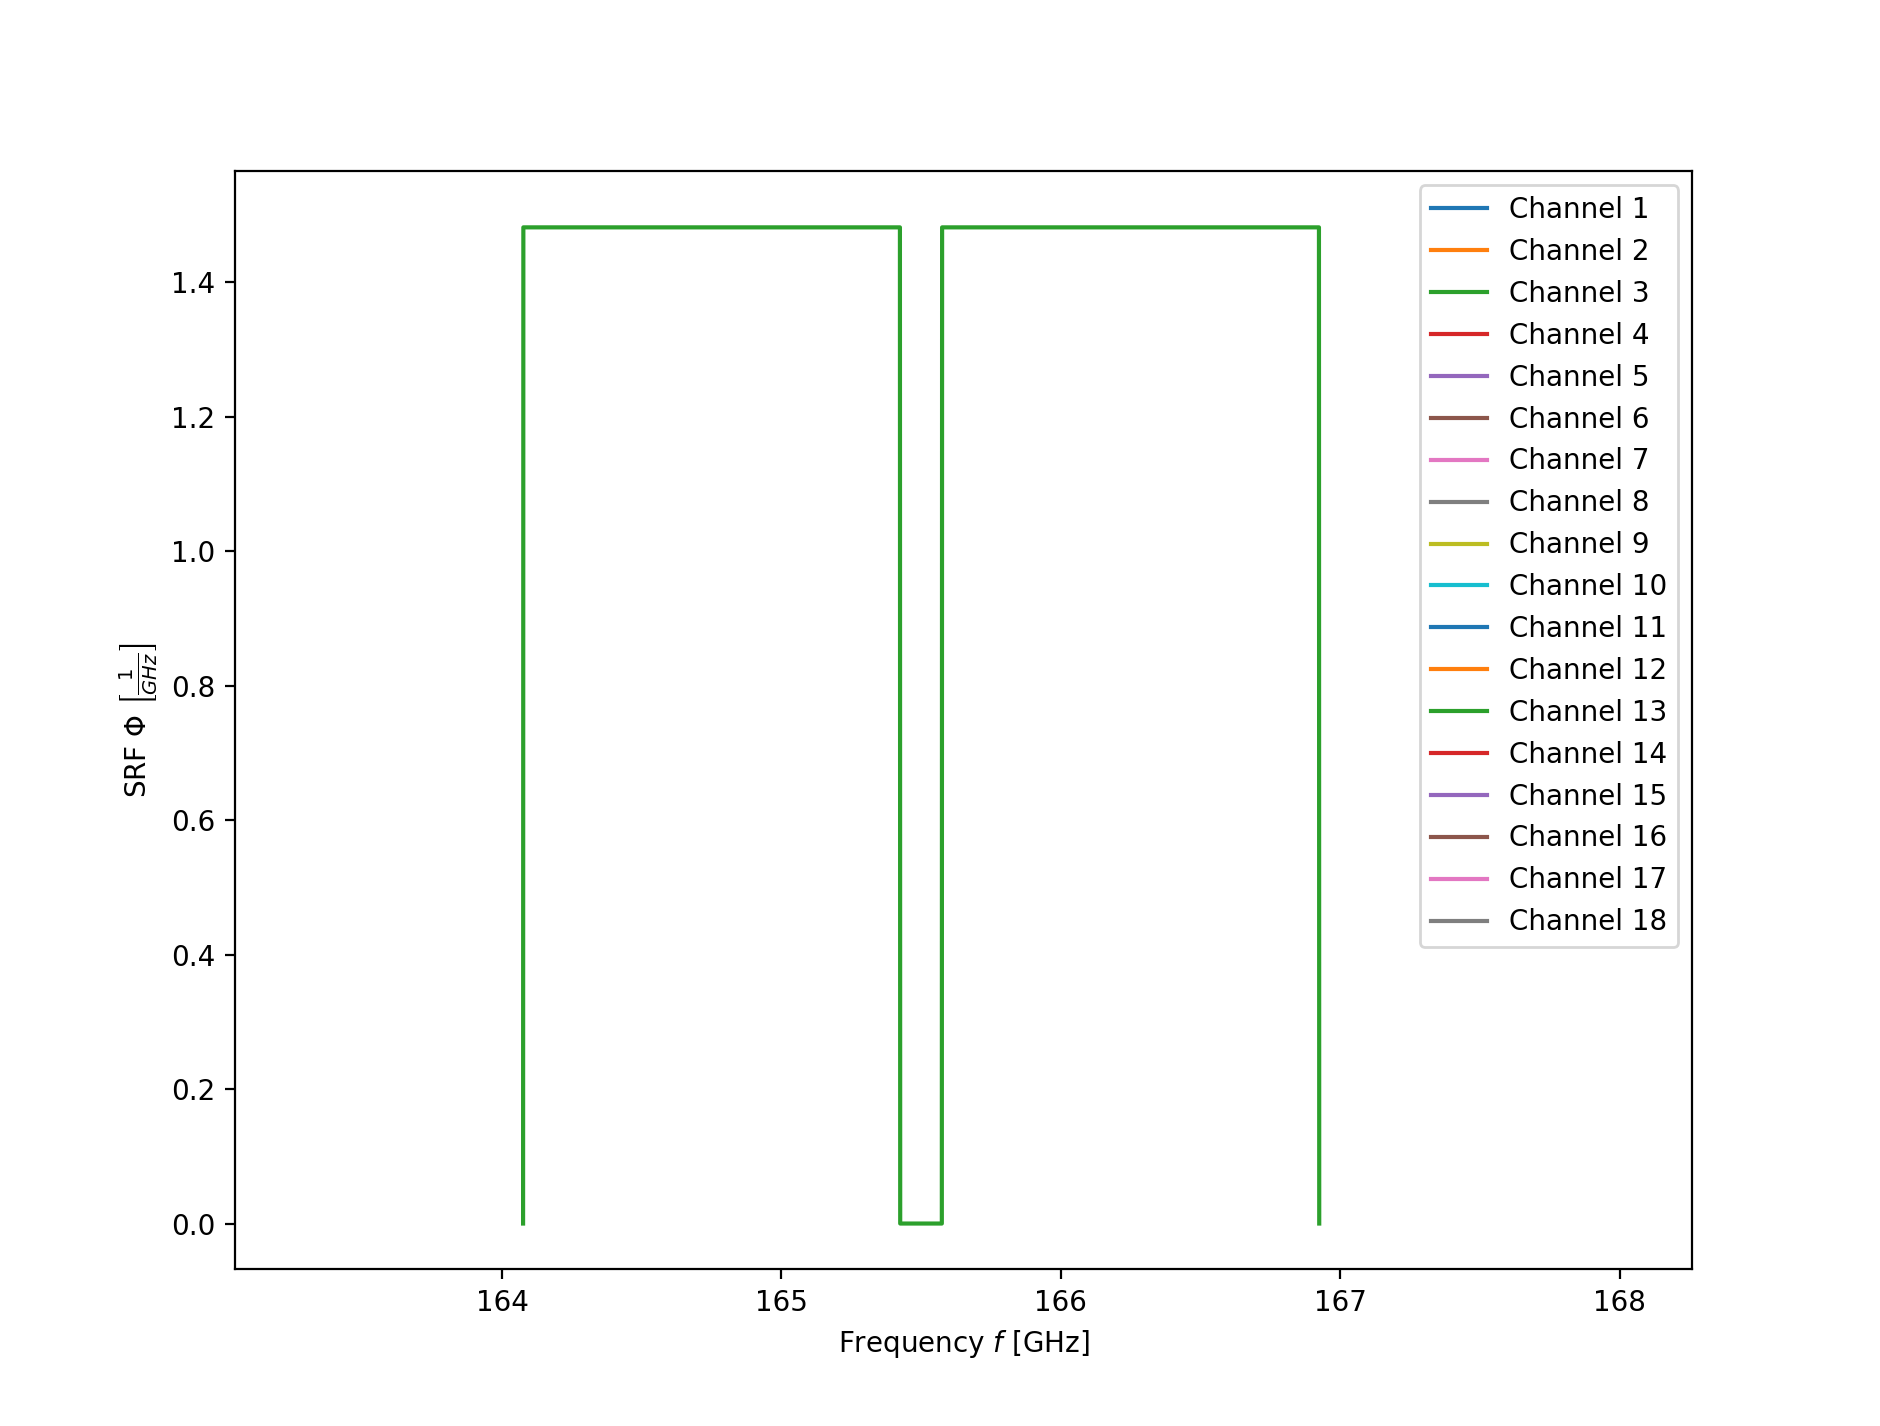
\includegraphics[width=\textwidth]{graphics/mwi_boxcar_zoom_ch13.png}
 \caption{Zoom on channel 13 boxcar SRF with two symmetric bands.}
 \label{fig:boxcar2}
 \end{figure}
 
  \begin{figure}[H]
 \centering
 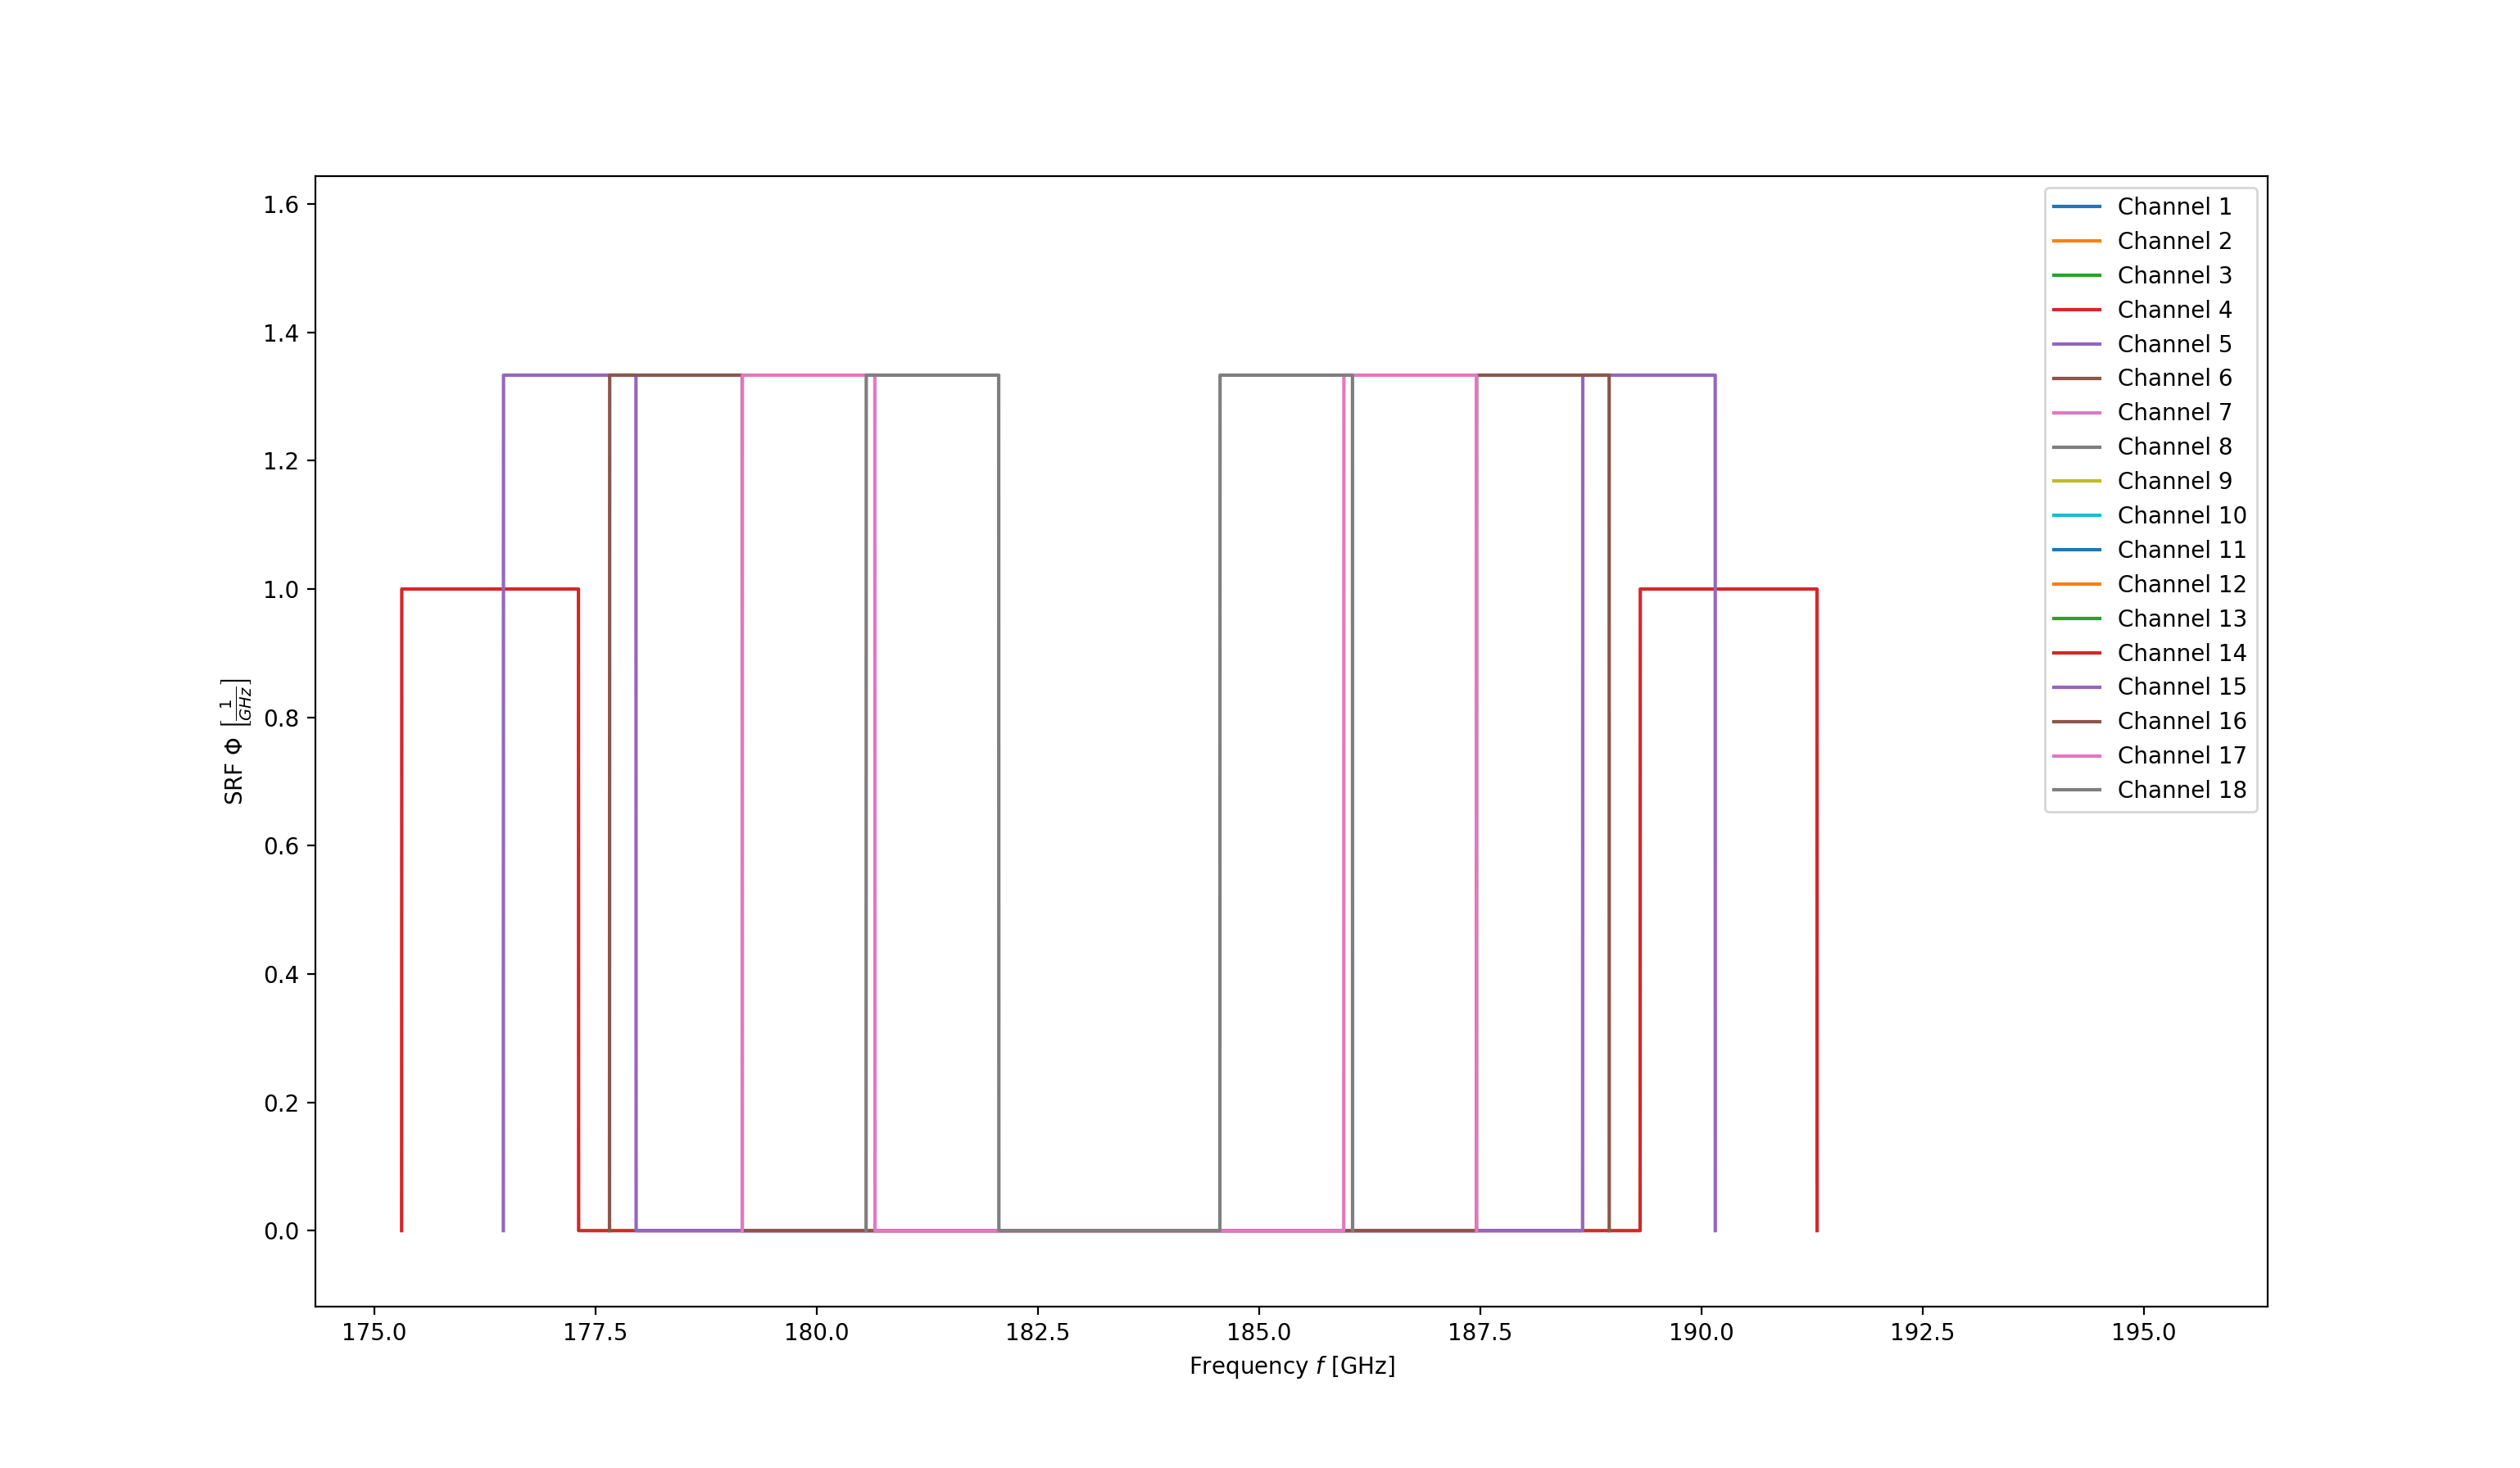
\includegraphics[width=\textwidth]{graphics/mwi_boxcar_zoom_183GHz.png}
 \caption{Zoom on the 183 GHz region with multiple overlapping channels..}
 \label{fig:boxcar3}
 \end{figure}
 
 \section{Coefficient Calculations}
 
 The microwave line-by-line calculations for the CRTM coefficients were performed using the CRTM-internal Rosenkranz'03 model at a resolution of 1 MHz, and for the coefficient regression the ODPS scheme was used.
 
 % The references section
%=======================
\clearpage
\bibliographystyle{plainnat}
\bibliography{bibliography}

\begin{thebibliography}{9}

\bibitem{mwi}
  V. Mattioli, C. Accadia, J. Ackermann, S. Di Michele, Imke Hans, P. Sch\"ussel, P. Colucci, and A Canestri
  \textit{ The EUMETSAT Polar System - Second Generation (EPS-SG) Passive Microwave and Sub-mm Wave Missions},
  Photonics and Electromagnetics Research Symposium,
  PIERS, Rome,
  2019.
  
 \end{thebibliography}

\end{document}

